\begin{enumerate}[label=\thesubsection.\arabic*.,ref=\thesubsection.\theenumi]
\numberwithin{equation}{enumi}

\item Consider the Magnitude Bode Plot and Phase Bode Plot \ref{fig:Bode} of Open-Loop Transfer Function of an Amplifier. Estimate the Open-Loop Transfer Function. (Assume $'A'$ as $'G'$ and $'\beta'$ as $'H'$)
\begin{figure}[ht!]
	\begin{center}
		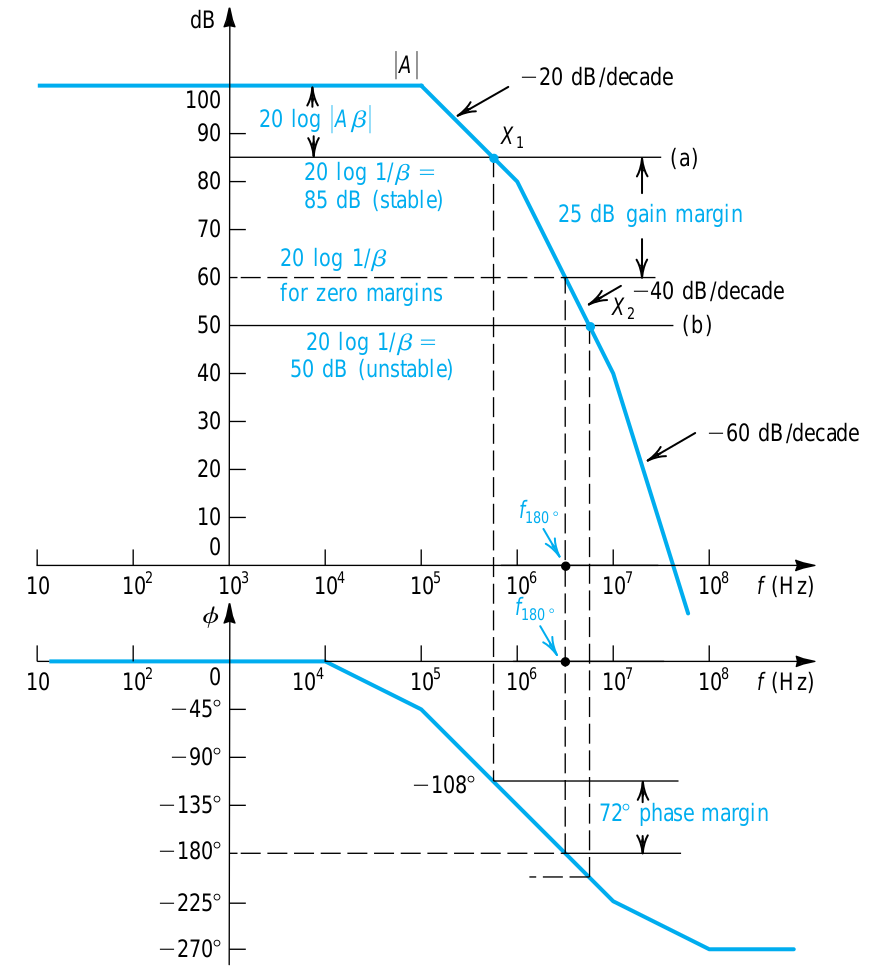
\includegraphics[width=\columnwidth]{./figs/ee18btech11014/ee18btech11014_figa.eps}
	\end{center}
	\caption{Magnitude and Phase Bode Plot}
	\label{fig:Bode}
\end{figure}\\
\solution Let $G(f)$ be the Open-Loop Transfer Function,
\begin{align}
G(f) = 
\begin{cases} 
      100 & 0 < f < 10^{5} \\
      200-20log(f) & 10^{5} < f < 10^{6} \\
      320-40log(f) & 10^{6} < f < 10^{7} \\
      460-60log(f) & 10^{7} < f  \\
\end{cases}
\end{align}

\begin{align}
\nabla G(f) &= \dfrac{d(G(f))}{d(log(f))} =
\begin{cases} 
        0 & 0 < f < 10^{5} \\
      -20 & 10^{5} < f < 10^{6} \\
      -40 & 10^{6} < f < 10^{7} \\
      -60 & 10^{7} < f  \\ 
\end{cases}
\end{align}

As we know that, \textbf{When a pole is encountered the slope always decreases by 20 dB/decade} and \textbf{When a zero is encountered the slope always increases by 20 dB/decade}. So, by observing \ref{fig:Bode} it can be concluded that we are having Poles at $f=10^{5} Hz, 10^{6} Hz, 10^{7} Hz$ and No Zeros.\\

So, the Open-Loop Transfer Function $G(f)$ is
\begin{align}
	G(f) = \dfrac{10^{5}}{\left(1+j\frac{f}{10^{5}}\right)\left(1+j\frac{f}{10^{6}}\right)\left(1+j\frac{f}{10^{7}}\right)}
\end{align}\\
%-------------------------------------------------------------------------------------------------%

\item Calculate the Phase of Open-Loop Transfer Function.\\
\solution\\
Phase of Open-Loop Transfer Function = $\phi$
\begin{align}
\phi=-\left[\tan ^{-1}\left(f / 10^{5}\right)+\tan ^{-1}\left(f / 10^{6}\right)+\tan ^{-1}\left(f / 10^{7}\right)\right]
\end{align}
%-------------------------------------------------------------------------------------------------%

%\item Determine on which Segment of Phase Bode Plot does $\phi = -180^{\circ}$\\
%\solution \\
%Assuming the Poles are widely spread, the phase is approximately $-45^{\circ}$ at the first pole frequency, $-135^{\circ}$ at the second, and $-225^{\circ}$ at the third. So, the phase is $-180^{\circ}$ between the Second and Third Pole or $10^{6} < f < 10^{7}$. So, the frequency at which the phase of $G(f)$ is $-180^{\circ}$ lies on the -40-dB/decade segment.\\
%-------------------------------------------------------------------------------------------------%

\item Determine the Closed-Loop Voltage Gain of the System assuming $|GH|\gg1$ and also assuming the block diagram of Control System is \ref{fig:Control}
\begin{figure}[ht!]
	\begin{center}
		\resizebox{\columnwidth/1}{!}{\begin{circuitikz}[american]
\ctikzset{tripoles/mos style/arrows}
\draw  (0,0) node[ground](GND){} -- (0,1) to[isource, l= $I_{s}$] (0,3) -- (2,3) to[R=$R_{F}$, i=$I_{f}$] (4,3) -- (6,3)node[label={right:C}]{} to[R=$R_{m}$] (6,0) node[ground](GND){} (6,0);

\draw (1,3) node[label={below:A}]{} to[short,i=$I_{i}$] (1,4);
\draw (1,6) node[label={right:B}]{} to[cisource, l= $-g_{m_{1}}v_{A}$] (1,4);
\draw (1,4) to[short, -o] (-1,4) node[label={above:$-$}]{} node[label={below:$S_{1}$}]{};
\draw (-1,5.5) node[label={below:$-v_{A}$}]{};
\draw (-2,6) node[label={below:$G_{1}$}]{} to[short, -o] (-1,6) node[label={below:$+$}]{};
\draw (1,6) to[R=$R_{D}$, i=$I_{i}$] (1,9);
\draw (1,9) node[ground,rotate=180](GND){} (1,9);

\draw (6,7) to[R=$R_{L}$,i=$I_{o}$] (6,3);
\draw (6,8) to[cisource, l= $-g_{m_{2}}v_{B}$] (6,7);
\draw (6,6.5) to[short, -o] (4,6.5) node[label={above:$-$}]{} node[label={below:$G_{2}$}]{};
\draw (4,8) node[label={below:$-v_{B}$}]{};
\draw (3,8.5) node[label={below:$S_{2}$}]{} to[short, -o] (4,8.5) node[label={below:$+$}]{};
\draw (6,7) -- (6,9);
\draw (6,9) node[ground,rotate=180](GND){} (6,9);

\end{circuitikz}
}
	\end{center}
	\caption{}
	\label{fig:Control}
\end{figure}

\solution\\
The Closed-Loop Voltage Gain of the Control System is\\
\begin{align}
T = \frac{V_{o}}{V_{s}} = \frac{G}{1+GH}
\end{align}

\begin{align}
20\log(T) = 20\log(G) - 20\log(1+GH)
\end{align}

Considering the assumption $|GH| \gg 1$, It can be written as
\begin{align}
20\log(1+GH) = 20\log(GH)
\end{align}

So,
\begin{align}
20\log(T) = 20\log(G) - 20\log(GH) \\
20\log(T) = -20\log(H) \\
20\log(T)= 20\log(\frac{1}{H})\\
T = \frac{1}{H}
\end{align}

So, The value of Closed-Loop Voltage Gain of the Control System under the assumption, $|GH| \gg 1$ is $T = \frac{1}{H}$\\
%-------------------------------------------------------------------------------------------------%

\item What is the value of Loop-Gain?\\
\solution\\
The value of Loop-Gain can be calculated by the difference of 2-curves $20\log|A|$ and $20log(\frac{1}{H})$. The difference between the two curves will be
\begin{align}
20 \log |G|-20 \log \frac{1}{H}=20 \log |GH|
\end{align}
%-------------------------------------------------------------------------------------------------%

\item Define Phase-Margin\\
\solution\\
\textbf{Phase-Margin:} The phase margin is defined as the angle in degrees by which the phase angle is smaller than $-180^{\circ}$ at the gain crossover, the gain crossover being the frequency at which the open-loop gain first reaches 1. \\
%-------------------------------------------------------------------------------------------------%

\item Find the frequencies for which phase margins are $90^{\circ}$ and $45^{\circ}$ respectively?\\
\solution\\
Let Phase Margin be $\alpha = 90^{\circ}$. Then,
\begin{align}
\alpha = \phi - (-180^{\circ})\\
\phi = -180^{\circ} + \alpha\\
\phi = -90^{\circ}
\end{align}

So, by the definition of Phase-Margin, at $\phi = -90^{\circ}$ , $|GH| = 1 $.  The value of $\phi = -90^{\circ}$ between poles $f=10^{5}Hz,10^{6}Hz$. Assuming the Poles are farther apart, 
\begin{align}
\tan^{-1}(\frac{f}{10^{7}}) \approx 0
\end{align}
where $10^{5} < f < 10^{6}$

So,
\begin{align}
-\tan^{-1}\left(f/10^{5}\right)-\tan^{-1}\left(f/10^{6}\right) = -90\\
\tan^{-1}\left(f/10^{5}\right)+\tan^{-1}\left(f/10^{6}\right) = 90\\
\tan^{-1}\left(f/10^{5}\right) = 90-\tan^{-1}\left(f/10^{6}\right)\\
\tan^{-1}\left(f/10^{5}\right) = \cot^{-1}\left(f/10^{6}\right)\\
\tan^{-1}\left(f/10^{5}\right) = \tan^{-1}\left(10^{6}/f\right)\\
f^{2} = 10^{11}\\
f = 3.162 \times 10^{5}
\end{align}

So, the approximate value of $f$ at which Phase Margin is $90^{\circ}$ is $f=3.162 \times 10^{5} Hz$.\\

Similarly let Phase Margin be $\alpha = 45^{\circ}$. Then,
\begin{align}
\alpha = \phi - (-180^{\circ})\\
\phi = -180^{\circ} + \alpha\\
\phi = -135^{\circ}
\end{align}

So, by the definition of Phase-Margin, at $\phi = -135^{\circ}$ , $|GH| = 1 $.  The value of $\phi = -135^{\circ}$ aproximately at poles $f=10^{6} Hz$. 

So, the approximate value of $f$ at which Phase Margin is $45^{\circ}$ is $f=10^{6}$.\\
%-------------------------------------------------------------------------------------------------%

\item Find the minimum values of Closed-Loop Voltage Gain for which phase margins are $90^{\circ}$ and  $45^{\circ}$ respectively\\
\solution\\
For $\alpha=90^{\circ}$,
\begin{align}
f=3.162 \times 10^{5}
\end{align}
By substituting $f$ in Open-Loop Gain $G(f)$ (assuming poles are far part), 
\begin{align}
G(f) = 200 - 20log(3.162 \times 10^{5})\\
G(f) = 90 dB \\
G = 3.1625 \times 10^{4}
\end{align}

At that $f=3.162 \times 10^{5}$, 
\begin{align}
H = \frac{1}{G}\\
H = 3.162 \times 10^{-5}
\end{align}

The minimum value of Closed-Loop Gain occurs at $|GH| \gg 1$ and the value of Closed-Loop Gain is $T=\frac{1}{H}$

\begin{align}
T = \frac{1}{H} = 3.1625 \times 10^{4}
\end{align}

\textbf{So, The minimum value of Closed-Loop Gain with Phase Margin equal to $\alpha=90^{\circ}$ is $T_{min} = 3.1625 \times 10^{4}$.}\\

For $\alpha=45^{\circ}$,
\begin{align}
f=10^{6}
\end{align}
By substituting $f$ in Open-Loop Gain $G(f)$ (assuming poles are far part), 
\begin{align}
G(f) = 200 - 20log(10^{6})\\
G(f) = 80 dB \\
G = 10^{4}
\end{align}

At that $f = 10^{6}$, 
\begin{align}
H = \frac{1}{G}\\
H = 10^{-4}
\end{align}

The minimum value of Closed-Loop Gain occurs at $|GH| \gg 1$ and the value of Closed-Loop Gain is $T=\frac{1}{H}$

\begin{align}
T = \frac{1}{H} = 10^{4}
\end{align}

\textbf{So, The minimum value of Closed-Loop Gain with Phase Margin equal to $\alpha=45^{\circ}$ is $T_{min} = 10^{4}$.}
%-------------------------------------------------------------------------------------------------%


\end{enumerate}
